\documentclass[10pt]{article}
\usepackage{upgreek}
\usepackage{amsmath}
\usepackage{graphicx}
\usepackage{subfig}
\usepackage{hyperref}
\usepackage{mathrsfs}
\usepackage{amssymb}
\usepackage{caption}
\usepackage{tikz}
\usepackage{verbatim}
\usetikzlibrary{shapes.geometric, arrows}

\tikzstyle{startstop} = [rectangle, rounded corners, minimum width=3cm, minimum height=1cm,text centered, draw=black, fill=red!30]
\tikzstyle{io} = [trapezium, trapezium left angle=70, trapezium right angle=110, minimum width=3cm, minimum height=1cm, text centered, draw=black, fill=blue!30]
\tikzstyle{process} = [rectangle, minimum width=3cm, minimum height=1cm, text centered, draw=black, fill=orange!30]
\tikzstyle{decision} = [diamond, minimum width=3cm, minimum height=1cm, text centered, draw=black, fill=green!30]
\tikzstyle{arrow} = [thick,->,>=stealth]

\DeclareGraphicsExtensions{.pdf,.png,.jpg,.tif}

\title{Reinforced Fiber Segmenation \\ Blob Detection }

\author{Sungmin Hong}
\date{\today}

\begin{document}
\maketitle

\section*{Summary of the Previous Report}
\label{prev}


The blob detection method using the ratio of Eigenvalues of Hessian matrix was experimented in the previous report(7\_OCT). 
The method depends solely on 2nd derivative of image apporximated by the LoG filter. 
Thus, the method is sensitive to $\sigma$ of LoG filter for detecting blobs and vessels.
Small $\sigma$ results in many false positives for blob detection, especially in vessels which have similar statistical property as blobs. 
On the contrary, large $\sigma$ misses small air blobs even though it is obvious in the sense of intensity. 
Most of vessel-like structure segmentation method set a single $\sigma$ for an entire image, which is inappropriate for air-voids detection. 
To solve the variation of the size of air-voids, I suggested methods which aid the 2nd derivative segmentation method by intensity-based segmentation, or clustering, methods.
I suggested the method using the maximally stable extremal regions(MSER) feature and K-Means clustering for the blob detection. 


\section*{Assumptions}
\label{assumption}

There are a few assumptions on air-voids that I made to detect air-voids from a concrete CT image. 
I do not know this would be always true for every CT image, but I tried to be careful since it restricts the problem.

\begin{enumerate}
 \item Darker than any other components(blocks and fibers) in CT image
 \item Uniformly distributed intensity, which means standard deviation of intensity in air-voids is small
 \item Blob-like shapes 
\end{enumerate}

\section*{Watershed segmentation and K-Means clustering method}
\label{methods}

\begin{figure}[h!tb]
  \centering
    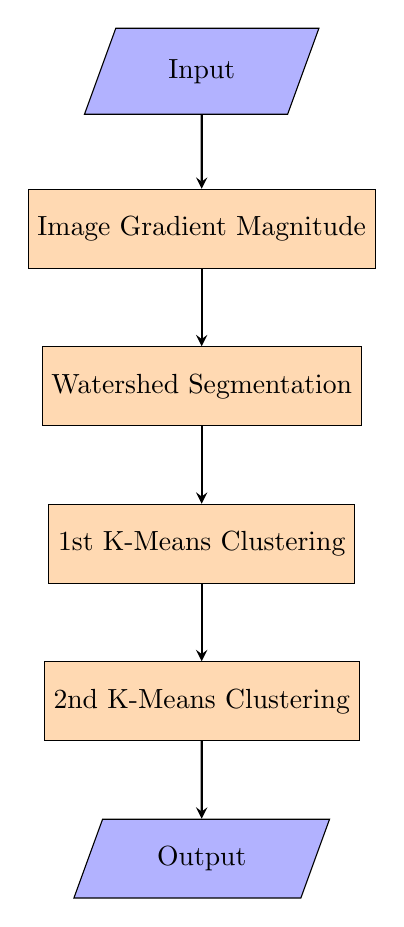
\begin{tikzpicture}[node distance=2cm]
    \node (in1) [io] {Input};
    \node (pro1) [process, below of=in1] {Image Gradient Magnitude};
    \node (pro2) [process, below of=pro1] {Watershed Segmentation};
    \node (pro3) [process, below of=pro2] {1st K-Means Clustering};
    \node (pro4) [process, below of=pro3] {2nd K-Means Clustering};
    \node (out1) [io, below of=pro4] {Output};

    \draw [arrow] (in1) -- (pro1);
    \draw [arrow] (pro1) -- (pro2);
    \draw [arrow] (pro2) -- (pro3);
    \draw [arrow] (pro3) -- (pro4);
    \draw [arrow] (pro4) -- (out1);
    \label{figFc}
    \end{tikzpicture}
  \caption{Overall work flow of the blob detection algorithm}
\end{figure}

By the first and the second assumptions, I tried the 1st derivative based watershed segmentation for detecting the blob candidates 
and intensity based K-means clustering method for grouping candidates by intensity distribution. Figure~\ref{figFc} describes the over all
flow of the current implemented algorithm.

First, we calculate the graident magnitude of an input image as a valley map for the watershed segmentation algorithm. 
The watershed algorithm with ``proper'' level and threshold generated blobs as shown in Figure~\ref{figGrW}. 

\begin{figure}[h!tb]
  \centering
  \captionsetup[subfigure]{labelformat=empty}
  \subfloat[Input]{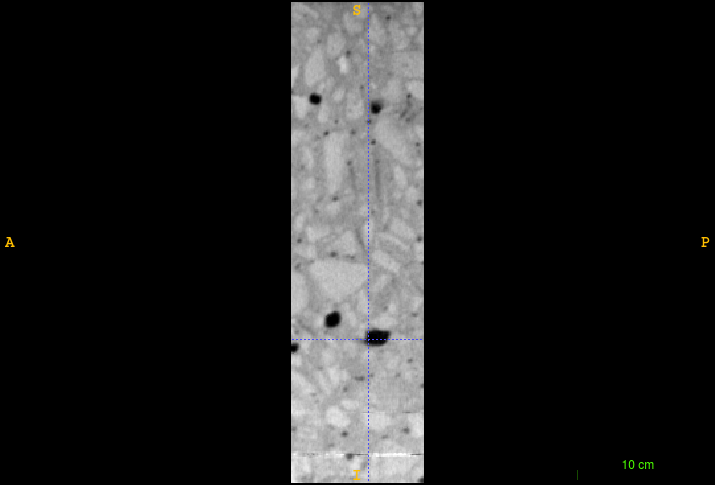
\includegraphics[width=40mm, height=40mm]{Image1.png}}  \hfill
  \subfloat[Gradient Magnitude]{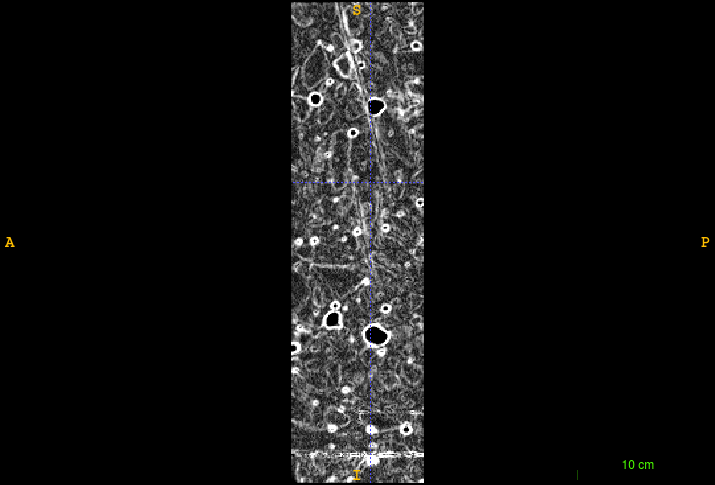
\includegraphics[width=40mm, height=40mm]{Gradient1.png}} \hfill
  \subfloat[Watershed]{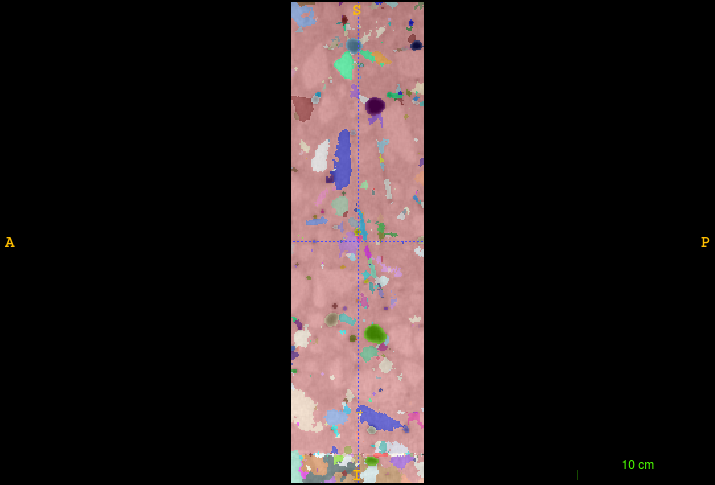
\includegraphics[width=40mm, height=40mm]{Watershed1.png}}  
\caption{Gradient magnitude image and watershed segmentation results}
\label{figGrW}
\end{figure}

I put the result of watershed algorithm into the K-means clustering method with $ K = 4 $, $K$ is decided by the observation to the input image. 
For K-means clustering, the Connected Component Analysis was used to group the adjacent object voxels. 
Then I extracted mean intensity, mean eigenvalues of Hessian matrix (I will discuss about the effect of $\sigma$ of LoG filter in the next section) for 
each component and put them into the clustering methods. As shown in Figure~\ref{figE}, the eigenvalues of each voxel have seperability for blobs.

\begin{figure}[h!tb]
  \centering
  \captionsetup[subfigure]{labelformat=empty}
  \subfloat[Input]{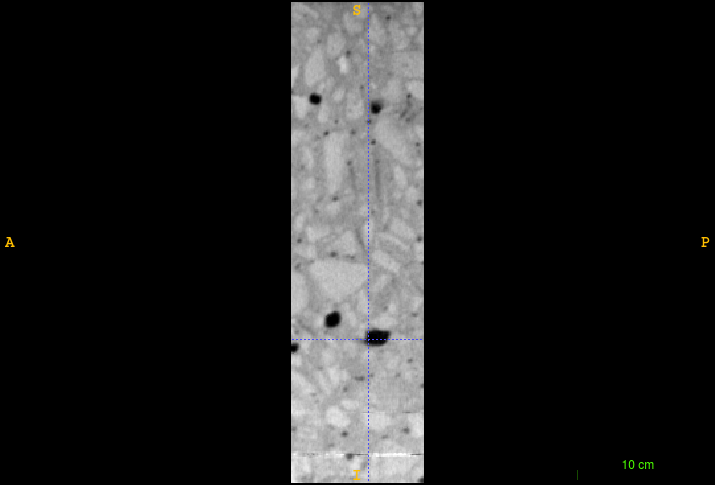
\includegraphics[width=40mm, height=40mm]{Image1.png}}  \hfill
  \subfloat[$\lambda_1$]{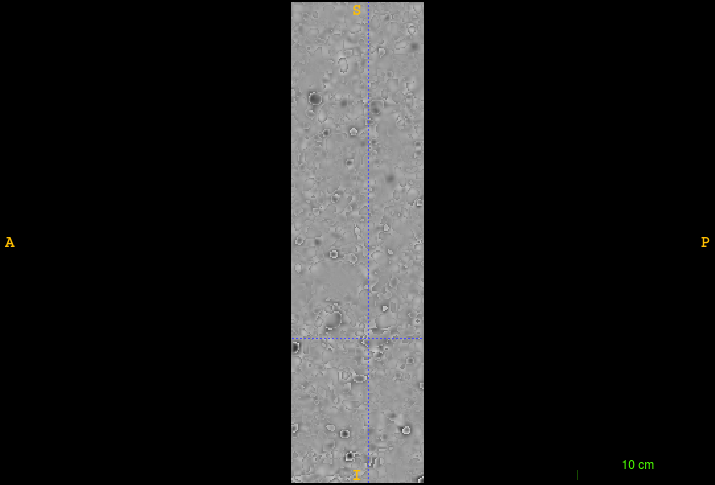
\includegraphics[width=40mm, height=40mm]{E0Sigma21.png}}  \hfill
  \subfloat[$\lambda_2$]{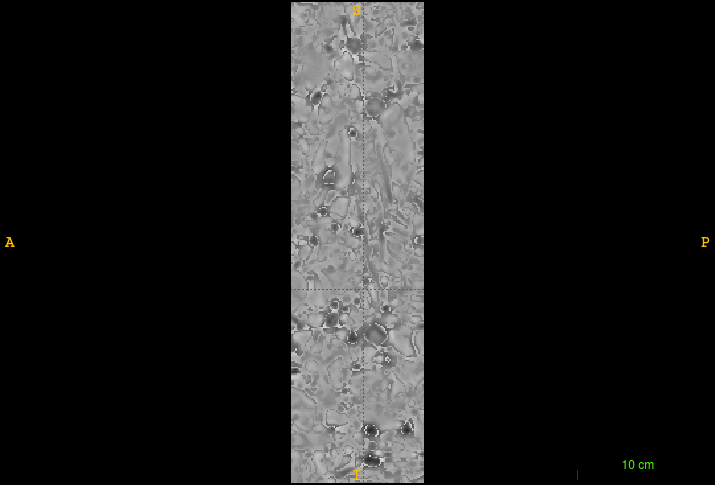
\includegraphics[width=40mm, height=40mm]{E1Sigma21.png}} \hfill
  \subfloat[$\lambda_3$]{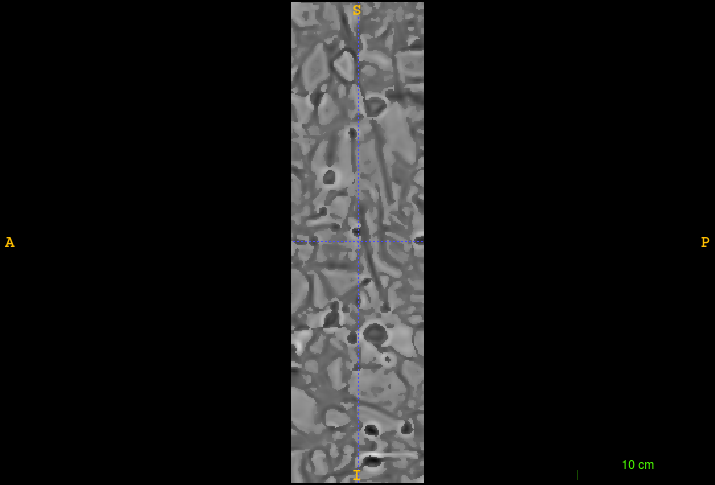
\includegraphics[width=40mm, height=40mm]{E2Sigma21.png}}  
\caption{Input features for 1st K-Means clustering. Intensity and eigenvalue maps of Hessian matrix for each voxel, $\lambda_1 < \lambda_2 < \lambda_3$}
\label{figE}
\end{figure}





\begin{comment}
\begin{figure}[h!tb]
  \centering
\captionsetup[subfigure]{labelformat=empty}
  \subfloat[Blobness $\sigma=2$]{\includegraphics[width=40mm, height=40mm]{BlobImage/Blobness2.png} } \hfill
  \subfloat[Blobness $\sigma=5$]{\includegraphics[width=40mm, height=40mm]{BlobSigma5/BlobnessPlane2.png}} \hfil
  \subfloat[Blobness $\sigma=10$]{\includegraphics[width=40mm, height=40mm]{BlobSigma10/Blobness.png}}  \\
  \subfloat[$\sigma=2, S_{th} =10$]{\includegraphics[width=40mm, height=40mm]{CCA_Min10/CCAPlane2.png} } \hfill
  \subfloat[$\sigma=2, S_{th} =100$]{\includegraphics[width=40mm, height=40mm]{CCA_Min100/CCAPlane2.png}} \hfil
  \subfloat[$\sigma=10, S_{th} =10$]{\includegraphics[width=40mm, height=40mm]{BlobSigma10/plane2Label.png}}  \\
\caption{Blobness $\mathcal{B}$ map generated with different $\sigma$ LoG filters}
\label{figBlobness}
\end{figure}

There can be two ways to detect differently sized blobs, $i)$ refining detected blob-like structures, or $ii)$ detecting structure-like regions and refining them by their shapes.
The refinement of detected blobs starts from over-segmented results of blobs with small $\sigma$, 
Since air-voids have low and almost uniform intensity compared to other objects in concrete, we may be able to apply clustering algorithms by intensity of blobs.
Then we select blobs in a cluster with lowest mean intensity. This method is expected to work well if over-segmentation of blobs captures all blobs and the nubmer of 
cluster classes is appropriate. 

The detection of structure-like regions followed by shape refinment starts from extracting maximally stable extreme regions(MSER) suggested by Matas et al. \cite{Matas02}.
Maximally stable extreme regions are defined solely by an extremal property of the intenstiy function in the region and on its outer boundary. It can be defined as regions 
which are stable over a large range of thresholds, when we slide threshold from the minimum intensity to the maximum intensity.
We extract extremal regions of image and conduct shape analysis to ROI for each candidate with different $\sigma$s or using the axis of geometric principal components.
Unlilke the shape analysis for an entire image, this method can have different $\sigma$s for each blob. 

Above two methods are based on the fact that air-voids are dark and have almost uniform intensity.
The methods may be hard to be generalized to other similar problems, such as, eliminating lesions for vein segmentation in a human liver, but this is just a far-away-future problem. 
I am currently working on the second method (MSER Shape Analysis) because I am not sure that the over-segmentation can guarantee capturing all air voids in the CT image. 
\end{comment}

\bibliographystyle{unsrt}
\bibliography{FRCBib.bib}

\end{document} 
